%  LaTeX support: latex@mdpi.com
%  For support, please attach all files needed for compiling as well as the log file, and specify your operating system, LaTeX version, and LaTeX editor.

%=================================================================
\documentclass[hydrology,article,submit,pdftex,moreauthors]{Definitions/mdpi}

% Additional packages
\usepackage{listings}
\usepackage{longtable}

% Code listing style
\lstset{
  basicstyle=\ttfamily\small,
  breaklines=true,
  frame=single,
  language=Python,
  numbers=left,
  numberstyle=\tiny\color{gray},
  keywordstyle=\color{blue},
  commentstyle=\color{green!50!black},
  stringstyle=\color{red!70!black},
  showstringspaces=false,
  xleftmargin=2em,
  framexleftmargin=1.5em
}

%=================================================================
% MDPI internal commands - do not modify
\firstpage{1}
\makeatletter
\setcounter{page}{\@firstpage}
\makeatother
\pubvolume{1}
\issuenum{1}
\articlenumber{0}
\pubyear{2026}
\copyrightyear{2026}
%\externaleditor{Academic Editor: Firstname Lastname}
\datereceived{ }
\daterevised{ }
\dateaccepted{ }
\datepublished{ }
\hreflink{https://doi.org/}

%=================================================================
% Full title of the paper (Capitalized)
\Title{PyBaseflow: A Python Package for Baseflow Separation Unifying Digital Filters, Graphical Methods, and Tracer-Based Approaches}

% MDPI internal command: Title for citation in the left column
\TitleCitation{PyBaseflow: A Python Package for Baseflow Separation}

% Author ORCID IDs
\newcommand{\orcidauthorA}{0000-0002-7597-2825} % Norman Jones

% Authors, for the paper (add full first names)
\Author{Xueyi Li~$^{1}$, Amin Aghababaei~$^{1}$, Ryan van der Heijden~$^{2}$, Eniola Webster-Esho~$^{3}$, Joshua Hart~$^{1}$, Amber Kunz~$^{1}$, Berkeley Berrett~$^{1}$, Norman Jones~$^{1,}$*\orcidA{}, Gus Williams~$^{1}$, Donna Rizzo~$^{2}$, and T.~Prabhakar Clement~$^{3}$}

% MDPI internal command: Authors, for metadata in PDF
\AuthorNames{Xueyi Li, Amin Aghababaei, Ryan van der Heijden, Eniola Webster-Esho, Joshua Hart, Amber Kunz, Berkeley Berrett, Norman Jones, Gus Williams, Donna Rizzo and T. Prabhakar Clement}

% MDPI internal command: Authors, for citation in the left column
\AuthorCitation{Li, X.; Aghababaei, A.; van der Heijden, R.; Webster-Esho, E.; Hart, J.; Kunz, A.; Berrett, B.; Jones, N.; Williams, G.; Rizzo, D.; Clement, T.P.}

% Affiliations / Addresses
\address{%
$^{1}$ \quad Civil and Construction Engineering, Brigham Young University, Provo, UT 84602, USA\\
$^{2}$ \quad Civil and Environmental Engineering, University of Vermont, Burlington, VT 05405, USA\\
$^{3}$ \quad Civil, Construction and Environmental Engineering, University of Alabama, Tuscaloosa, AL 35487, USA}

% Contact information of the corresponding author
\corres{Correspondence: njones@byu.edu; Tel.: +1-801-225-0799 (N.J.)}

%\simplesumm{}

%\conference{}

% Abstract (Do not insert blank lines, i.e. \\)
\abstract{Baseflow---the portion of streamflow sustained by groundwater discharge---is fundamental to watershed hydrology, water resource management, and ecological assessment. Because baseflow cannot be measured directly, it must be estimated by separating it from total streamflow. Numerous separation methods exist, but they are scattered across legacy Fortran programs, web tools, and research scripts with inconsistent interfaces. We present \texttt{pybaseflow}, an open-source Python package that unifies 17 baseflow separation methods spanning four methodological paradigms: recursive digital filters (both linear-reservoir-based and signal-processing-based families), graphical and recession-based methods, and tracer-based approaches. A key contribution is the identification of a generalized three-parameter recursive digital filter equation that subsumes all 11 implemented recursive filters as special cases, revealing previously undocumented algebraic relationships among popular methods. The package also introduces the first Python implementation of the PART method, a conductivity mass balance (CMB) tracer module, and a CMB-to-Eckhardt calibration bridge linking physical measurements to digital filter parameters. Built on NumPy with Numba acceleration, \texttt{pybaseflow} provides a consistent function-oriented API, built-in USGS data retrieval, and comprehensive documentation. The package is pip-installable and available under the MIT license.}

% Keywords
\keyword{baseflow separation; digital filter; Python; open-source software; recession analysis; streamflow; tracer; hydrology}

%%%%%%%%%%%%%%%%%%%%%%%%%%%%%%%%%%%%%%%%%%
\begin{document}

%%%%%%%%%%%%%%%%%%%%%%%%%%%%%%%%%%%%%%%%%%
\section{Introduction}
\label{sec:introduction}

Streamflow comprises two primary components: quickflow, which responds rapidly to precipitation and snowmelt events, and baseflow, which represents the slower, sustained contribution from groundwater discharge, bank storage, and other delayed sources. Baseflow is critical for sustaining river ecosystems during dry periods, supporting water supply planning, and calibrating hydrological models~\cite{ChapmanMaxwell1996,Eckhardt2005}. However, baseflow cannot be measured directly in the field~\cite{ChapmanMaxwell1996}, so practitioners rely on separation methods to estimate it from observed total streamflow records.

Over several decades, a diverse array of separation methods has been developed, which can be broadly organized into four categories. \textit{Recursive digital filters} apply signal-processing or linear-reservoir-based equations to partition the hydrograph into baseflow and quickflow components~\cite{Lyne1979,Chapman1991,Eckhardt2005}. \textit{Graphical methods} identify baseflow through geometric rules applied to the hydrograph, such as fixed intervals, sliding windows, or local minima~\cite{Sloto1996}. \textit{Recession-based methods} exploit the characteristic exponential decay of baseflow during dry periods to anchor separation points~\cite{Rutledge1998}. \textit{Tracer-based methods} use hydrochemical measurements, such as specific conductance, to quantify the groundwater fraction via mass balance~\cite{Stewart2007}.

Despite the abundance of methods, practitioners face practical barriers to applying them. The USGS programs HYSEP~\cite{Sloto1996} and PART~\cite{Rutledge1998} are written in legacy Fortran and are difficult to integrate into modern analytical workflows. The Web-based Hydrograph Analysis Tool (WHAT)~\cite{Lim2005} provides a graphical interface but cannot be scripted or automated. Several R packages exist but are limited to a small subset of methods. The Python package by Xie et al.~\cite{Xie2020} implemented 11 digital filters but was designed primarily as research code for a specific comparative study, bundling geospatial and study-specific functionality that limited its reusability as a general-purpose library.

To address these gaps, we present \texttt{pybaseflow}, an open-source Python package that provides a unified, consistent interface to 17 baseflow separation methods across all four methodological paradigms. The package builds on the work of Xie et al.~\cite{Xie2020} but has been extensively refactored: study-specific code has been removed, four new methods have been added (PART, CMB, IHACRES, and BFlow), a new tracer module has been introduced, and the recursive digital filters have been unified under a single generalized equation. The result is a focused, pip-installable library with a flat, function-oriented API, built-in USGS data retrieval, Numba-accelerated performance, and comprehensive documentation.

This paper is organized as follows. Section~\ref{sec:framework} presents the theoretical framework, including the generalized recursive digital filter equation and descriptions of all implemented methods. Section~\ref{sec:design} describes the software architecture and implementation. Section~\ref{sec:examples} demonstrates usage through worked examples. Section~\ref{sec:discussion} discusses the package in context, including limitations and future directions. Section~\ref{sec:conclusions} concludes.

%%%%%%%%%%%%%%%%%%%%%%%%%%%%%%%%%%%%%%%%%%
\section{Theoretical Framework}
\label{sec:framework}

\subsection{Generalized Recursive Digital Filter}
\label{sec:generalized_filter}

A central contribution of this work is the observation that all 11 recursive digital filter methods implemented in \texttt{pybaseflow} can be expressed as special cases of a single three-parameter equation:
\begin{equation}
\label{eq:generalized}
b_t = \alpha \, b_{t-1} + \beta \left( Q_t + \gamma \, Q_{t-1} \right), \quad \text{subject to} \quad b_t \leq Q_t
\end{equation}
where $b_t$ is the estimated baseflow at time $t$, $Q_t$ is the observed streamflow, and $\alpha$, $\beta$, $\gamma$ are method-specific coefficients derived from the physical or empirical parameters of each method. The constraint $b_t \leq Q_t$ ensures that baseflow never exceeds total streamflow.

The parameter $\gamma$ divides the filters into two structural families. When $\gamma = 0$, the filter depends only on the current streamflow $Q_t$ and the previous baseflow $b_{t-1}$; these filters are grounded in linear reservoir theory. When $\gamma = 1$, the filter incorporates both $Q_t$ and $Q_{t-1}$, reflecting a signal-processing origin where the moving average of streamflow is used. Table~\ref{tab:coefficients} summarizes the coefficient mappings for all recursive filters.

\begin{table}[H]
\caption{Coefficient mappings for the generalized recursive digital filter (Equation~\ref{eq:generalized}). Each named method is a special case defined by its $\alpha$, $\beta$, and $\gamma$ values.\label{tab:coefficients}}
\small
\begin{tabularx}{\textwidth}{lccccl}
\toprule
\textbf{Method} & $\boldsymbol{\alpha}$ & $\boldsymbol{\beta}$ & $\boldsymbol{\gamma}$ & \textbf{Source Parameters} & \textbf{Reference} \\
\midrule
\multicolumn{6}{l}{\textit{Family 1: Linear reservoir filters ($\gamma = 0$)}} \\
\addlinespace
Chapman--Maxwell & $\dfrac{a}{2-a}$ & $\dfrac{1-a}{2-a}$ & 0 & $a$ & \cite{ChapmanMaxwell1996} \\[6pt]
Boughton & $\dfrac{a}{1+C}$ & $\dfrac{C}{1+C}$ & 0 & $a, C$ & \cite{Boughton1993} \\[6pt]
Eckhardt & $\dfrac{(1-\mathrm{BFI_{max}})a}{1-a \cdot \mathrm{BFI_{max}}}$ & $\dfrac{(1-a)\mathrm{BFI_{max}}}{1-a \cdot \mathrm{BFI_{max}}}$ & 0 & $a, \mathrm{BFI_{max}}$ & \cite{Eckhardt2005} \\[6pt]
EWMA & $1-e$ & $e$ & 0 & $e$ & \cite{Tularam2008} \\[6pt]
Furey--Gupta & $a - A(1-a)$ & $A(1-a)$ & 0 & $a, A$ & \cite{Furey2001} \\[6pt]
WHAT & \multicolumn{4}{l}{Alias for Eckhardt~\cite{Eckhardt2005}} & \cite{Lim2005} \\
\addlinespace
\midrule
\multicolumn{6}{l}{\textit{Family 2: Signal-processing filters ($\gamma = 1$)}} \\
\addlinespace
Lyne--Hollick & $\beta_p$ & $\dfrac{1-\beta_p}{2}$ & 1 & $\beta_p$ & \cite{Lyne1979} \\[6pt]
Chapman (1991) & $\dfrac{3a-1}{3-a}$ & $\dfrac{1-a}{3-a}$ & 1 & $a$ & \cite{Chapman1991} \\[6pt]
Willems & $\dfrac{a-v}{1+v}$ & $\dfrac{v}{1+v}$ & 1 & $a, w$ & \cite{Willems2009} \\
\addlinespace
\midrule
\multicolumn{6}{l}{\textit{Hybrid: Variable $\gamma$ ($-1 < \gamma < 0$)}} \\
\addlinespace
IHACRES & $\dfrac{a}{1+C}$ & $\dfrac{C}{1+C}$ & $\alpha_s$ & $a, C, \alpha_s$ & \cite{Jakeman1993} \\
\bottomrule
\end{tabularx}
\raggedright
\footnotesize{Note: For Willems, $v = \frac{(1-w)(1-a)}{2w}$ where $w$ is the quickflow fraction. For Furey--Gupta, $\beta$ operates on $Q_{t-1}$ rather than $Q_t$ (a lagged formulation).}
\end{table}

This unification reveals several important relationships. The Eckhardt filter is algebraically equivalent to the Boughton filter under the parameter transformation $C = (1-a) \cdot \mathrm{BFI_{max}} / (1 - \mathrm{BFI_{max}})$. When $\mathrm{BFI_{max}} = 0.5$, the Eckhardt filter further reduces to the Chapman--Maxwell filter. The IHACRES filter, with its variable $\gamma = \alpha_s$ parameter, bridges the two families: when $\alpha_s = 0$ it reduces to the Boughton filter ($\gamma = 0$ family), and as $\alpha_s \to -1$ it approaches the behavior of the $\gamma = 1$ family (Figure~\ref{fig:ihacres_sensitivity}).

The multi-pass Lyne--Hollick variant~\cite{Spongberg2000} applies the single-pass filter iteratively, alternating forward and backward passes. Each additional pass further smooths the baseflow estimate and reduces the baseflow index (BFI), as illustrated in Figure~\ref{fig:lh_passes}.

\begin{figure}[H]
\centering
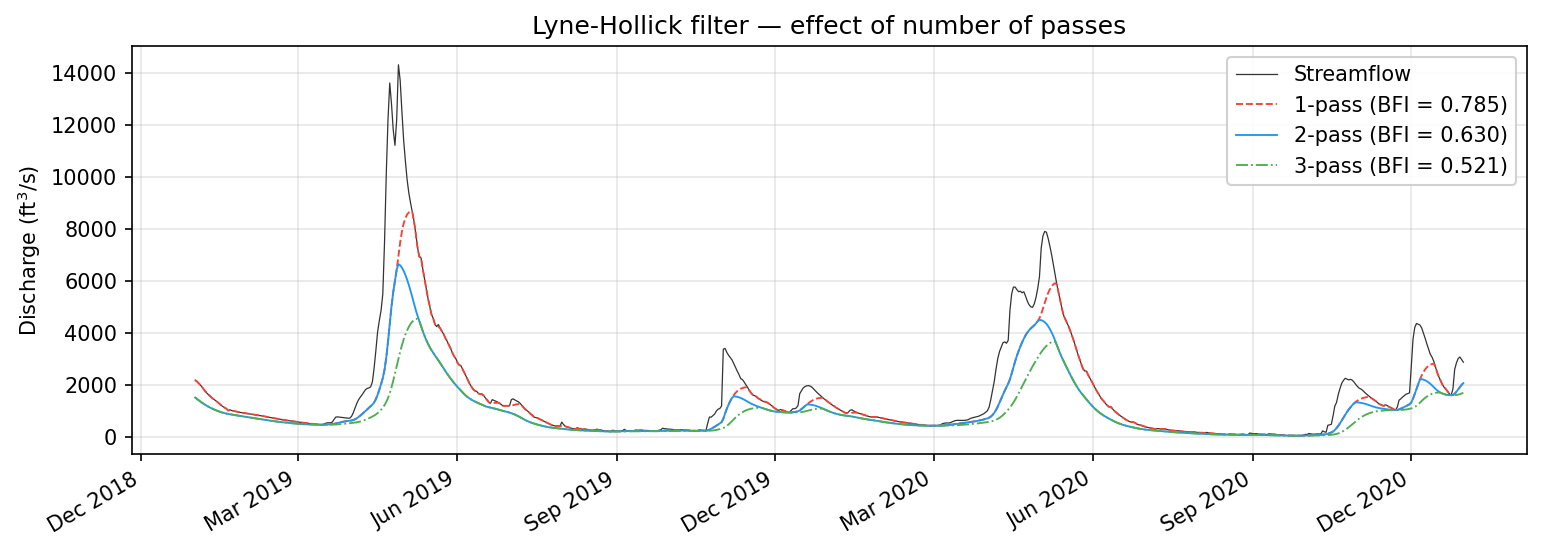
\includegraphics[width=0.85\textwidth]{figures/lyne_hollick_passes.png}
\caption{Effect of multiple passes of the Lyne--Hollick filter. Each additional pass produces a lower baseflow estimate and reduced BFI.\label{fig:lh_passes}}
\end{figure}

\subsection{Graphical and Recession-Based Methods}
\label{sec:graphical}

Graphical methods partition the hydrograph using geometric rules rather than recursive equations. The package implements five such methods.

\subsubsection{HYSEP Methods}

The three HYSEP methods~\cite{Sloto1996} use a drainage-area-dependent interval
$N^*$, computed as the nearest odd integer $\geq 2\lfloor A^{0.2}\rfloor + 1$,
where $A$ is the drainage area in square miles.

The \textit{fixed interval} method divides the record into non-overlapping blocks of $N^*$ days and assigns the minimum streamflow in each block as baseflow for the entire interval, producing a characteristic staircase pattern. The \textit{sliding interval} method applies a moving window of width $N^*$, assigning the window minimum to the central day, producing a smoother envelope. The \textit{local minimum} method identifies days that are local minima within the $N^*$-day window and connects them by linear interpolation.

\subsubsection{UKIH Smoothed Minima Method}

The UK Institute of Hydrology method~\cite{UKIH1980} divides the record into non-overlapping 5-day blocks and selects the minimum flow in each block. A turning point is retained only if it satisfies the screening criterion:
\begin{equation}
\label{eq:ukih}
0.9 \, Q_{\min,i} < Q_{\min,i-1} \quad \text{and} \quad 0.9 \, Q_{\min,i} < Q_{\min,i+1}
\end{equation}
Baseflow is obtained by linearly interpolating between retained turning points.

\subsubsection{PART Method}

The PART method~\cite{Rutledge1998}, implemented here in Python for the first time, identifies ``antecedent recession'' days where streamflow has been declining for at least $N = A^{0.2}$ days (with $N$ derived from the log-cycle criterion of Barnes~\cite{Barnes1939}). At these anchor points, baseflow is set equal to streamflow. Between anchor points, baseflow is interpolated in log-space:
\begin{equation}
\label{eq:part}
\log_{10}(b_t) = \log_{10}(b_{t_0}) + \frac{t - t_0}{t_1 - t_0} \left[ \log_{10}(b_{t_1}) - \log_{10}(b_{t_0}) \right]
\end{equation}
The method iterates, progressively relaxing the recession requirement until the number of anchor points stabilizes.

\subsection{Recession Analysis}
\label{sec:recession}

\subsubsection{BFlow Method}

The BFlow method~\cite{Arnold1999} estimates the SWAT model's baseflow recession constant (ALPHA\_BF) by fitting the exponential recession model:
\begin{equation}
\label{eq:bflow}
Q_b(t) = Q_b(0) \cdot e^{-\alpha t}
\end{equation}
The method applies the three-pass Lyne--Hollick filter and then performs linear regression on $\ln Q_b$ versus $t$ during identified recession periods. The resulting $\alpha$ yields the number of baseflow days as $\mathrm{BF_{days}} = \ln(10)/\alpha$.

\subsubsection{Brutsaert--Nieber (BN77) Method}

The BN77 method~\cite{Cheng2016} identifies drought-flow data points suitable for recession analysis by applying a series of elimination criteria to the recession slope $S(t) = (Q_{t-1} - Q_{t+1})/2$. Points surviving all filters represent pure baseflow conditions.

\subsection{Tracer-Based Methods}
\label{sec:tracer}

\subsubsection{Conductivity Mass Balance (CMB)}

The conductivity mass balance method~\cite{Stewart2007} separates baseflow using specific conductance (SC) as a conservative tracer. From the two-component mass balance:
\begin{equation}
\label{eq:cmb}
Q_b(t) = Q(t) \cdot \frac{SC(t) - SC_{RO}}{SC_{BF} - SC_{RO}}
\end{equation}
where $SC_{BF}$ and $SC_{RO}$ are the end-member specific conductance values for baseflow and runoff, respectively. End-members can be supplied by the user or estimated automatically from the data.

\subsubsection{CMB-to-Eckhardt Calibration Bridge}

A novel feature of the package is the ability to calibrate the Eckhardt filter's $\mathrm{BFI_{max}}$ parameter from tracer-derived baseflow, linking physical measurements to digital filter parameters. This follows the approach suggested by Stewart et al.~\cite{Stewart2007}, with the caveat noted by Zhang et al.~\cite{Zhang2021} that such calibration performs well at annual time scales (NSE~0.91--1.00) but can degrade at daily time scales (mean NSE of $-0.30$ across 26 stations).

%%%%%%%%%%%%%%%%%%%%%%%%%%%%%%%%%%%%%%%%%%
\section{Software Design and Implementation}
\label{sec:design}

\subsection{Package Architecture}
\label{sec:architecture}

The \texttt{pybaseflow} package (version 0.1.1) is organized into five modules:

\begin{itemize}[nosep]
\item \texttt{separation.py} --- All 17 separation method functions plus the shared computational core.
\item \texttt{estimate.py} --- Recession coefficient estimation, parameter calibration, BFI estimation, and BFlow recession analysis.
\item \texttt{tracer.py} --- CMB separation, end-member estimation, and the CMB-to-Eckhardt calibration bridge.
\item \texttt{io.py} --- USGS NWIS daily streamflow retrieval via \texttt{fetch\_usgs()}.
\item \texttt{utils.py} --- Preprocessing utilities including \texttt{clean\_streamflow()}, \texttt{moving\_average()}, and array helpers.
\end{itemize}

All public separation functions are importable from the top-level namespace (e.g., \texttt{import pybaseflow; b = pybaseflow.eckhardt(Q, a, BFImax)}) or from their respective submodules. Every separation function accepts a NumPy array \texttt{Q} and returns a NumPy array of the same length containing the estimated baseflow.

\subsection{Unified Filter Core}
\label{sec:filter_core}

The 11 recursive digital filters are implemented through a shared function, \texttt{\_recursive\_digital\_filter()}, which evaluates Equation~\ref{eq:generalized}. Each named method (e.g., \texttt{eckhardt()}, \texttt{chapman()}) is a thin wrapper that computes its specific $\alpha$, $\beta$, $\gamma$ coefficients from the user-supplied parameters and delegates to this shared function. This design eliminates code duplication, ensures consistent behavior, and makes the algebraic relationships between filters explicit in the implementation.

All filter methods accept an \texttt{initial\_method} parameter for setting $b_0$, with options including \texttt{'Q0'} (first streamflow value), \texttt{'min'} (minimum streamflow), \texttt{'LH'} (initial Lyne--Hollick estimate), or a user-specified constant. An optional \texttt{return\_exceed} flag reports the number of timesteps where the unconstrained filter produced $b_t > Q_t$.

\subsection{Data Input and Preprocessing}
\label{sec:data_input}

The \texttt{fetch\_usgs()} function in the \texttt{io} module retrieves daily streamflow data from the USGS National Water Information System (NWIS) using only the Python standard library (\texttt{urllib}, \texttt{json}). It accepts a site number, start date, and end date, and returns a pandas Series indexed by date:

\begin{lstlisting}
from pybaseflow.io import fetch_usgs
Q = fetch_usgs("01013500", start="2019-01-01", end="2020-12-31")
\end{lstlisting}

The \texttt{clean\_streamflow()} function preprocesses raw data by removing NaN values, filtering years with fewer than 120 valid days, and sorting chronologically. The package also bundles a sample dataset (USGS station 01013500, Fish River near Fort Kent, Maine, 2019--2020) accessible via \texttt{pybaseflow.load\_sample\_data()}, providing a snowmelt-dominated regime with a strong seasonal cycle suitable for demonstrating all methods.

\subsection{Performance Optimization}
\label{sec:performance}

Several computationally intensive functions, particularly the graphical method interpolation loops and parameter calibration routines, use Numba's \texttt{@njit} decorator for just-in-time compilation to machine code. Batch operations use \texttt{@njit(parallel=True)} with \texttt{prange} for multi-core acceleration.

\subsection{Dependencies and Installation}
\label{sec:dependencies}

The package requires Python $\geq$ 3.9 and depends on three core libraries: NumPy, pandas, and Numba. It is installable via:

\begin{lstlisting}[numbers=none]
pip install pybaseflow
\end{lstlisting}

The source code is hosted at \url{https://github.com/BYU-Hydroinformatics/pybaseflow} under the MIT license. Documentation built with MkDocs is available at \url{https://pybaseflow.readthedocs.io/en/latest/}, including method guides with equations and figures, practical tutorials, and auto-generated API reference.

%%%%%%%%%%%%%%%%%%%%%%%%%%%%%%%%%%%%%%%%%%
\section{Usage Examples}
\label{sec:examples}

This section demonstrates the package workflow using the bundled Fish River dataset (USGS 01013500, 2019--2020).

\subsection{Basic Separation}
\label{sec:basic_example}

A complete baseflow separation requires only a few lines of code:

\begin{lstlisting}[caption={Basic usage: loading data and applying a separation method.},label={lst:basic}]
import pybaseflow
import numpy as np

# Load bundled sample data (Fish River, Maine)
Q, dates = pybaseflow.load_sample_data()

# Estimate recession coefficient
from pybaseflow.estimate import recession_coefficient
a = recession_coefficient(Q)

# Apply a separation method
b = pybaseflow.eckhardt(Q, a=a, BFImax=0.80)

# Calculate baseflow index
BFI = np.sum(b) / np.sum(Q)
\end{lstlisting}

Figure~\ref{fig:eckhardt} shows the Eckhardt separation result, with baseflow shown as the shaded area beneath the streamflow hydrograph.

\begin{figure}[H]
\centering
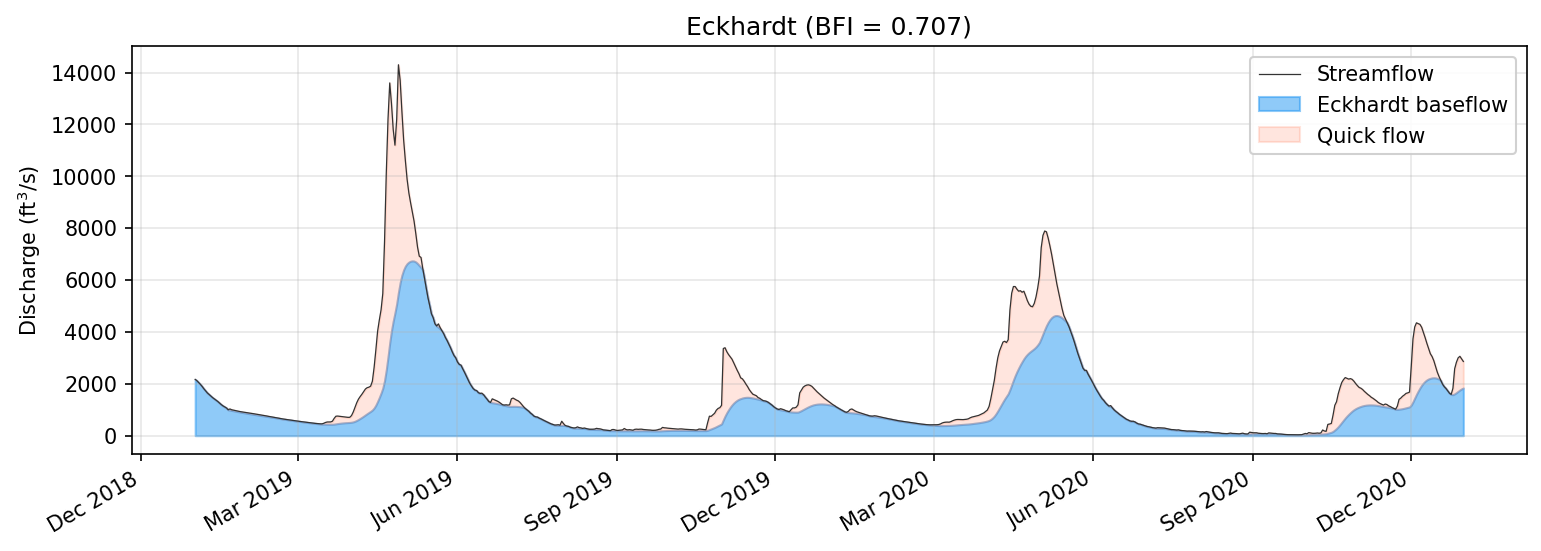
\includegraphics[width=0.85\textwidth]{figures/eckhardt.png}
\caption{Eckhardt filter baseflow separation applied to Fish River (USGS 01013500), 2019--2020. Shaded area represents estimated baseflow; unshaded area represents quickflow.\label{fig:eckhardt}}
\end{figure}

\subsection{Comparing Multiple Methods}
\label{sec:comparison}

Because all methods share a consistent API, comparing them is straightforward:

\begin{lstlisting}[caption={Applying multiple separation methods for comparison.},label={lst:compare}]
from pybaseflow.separation import (eckhardt, chapman, lh,
    fixed, ukih, part)

results = {
    'Eckhardt':  eckhardt(Q, a=a, BFImax=0.80),
    'Chapman':   chapman(Q, a=a),
    'Lyne-Hollick': lh(Q),
    'Fixed':     fixed(Q, area=1430),
    'UKIH':      ukih(Q, b_LH=lh(Q)),
    'PART':      part(Q, area=1430),
}
\end{lstlisting}

Figure~\ref{fig:overview} presents an overview comparison of all 17 methods applied to the Fish River dataset, illustrating the range of baseflow estimates and BFI values produced by different approaches.

\begin{figure}[H]
\centering
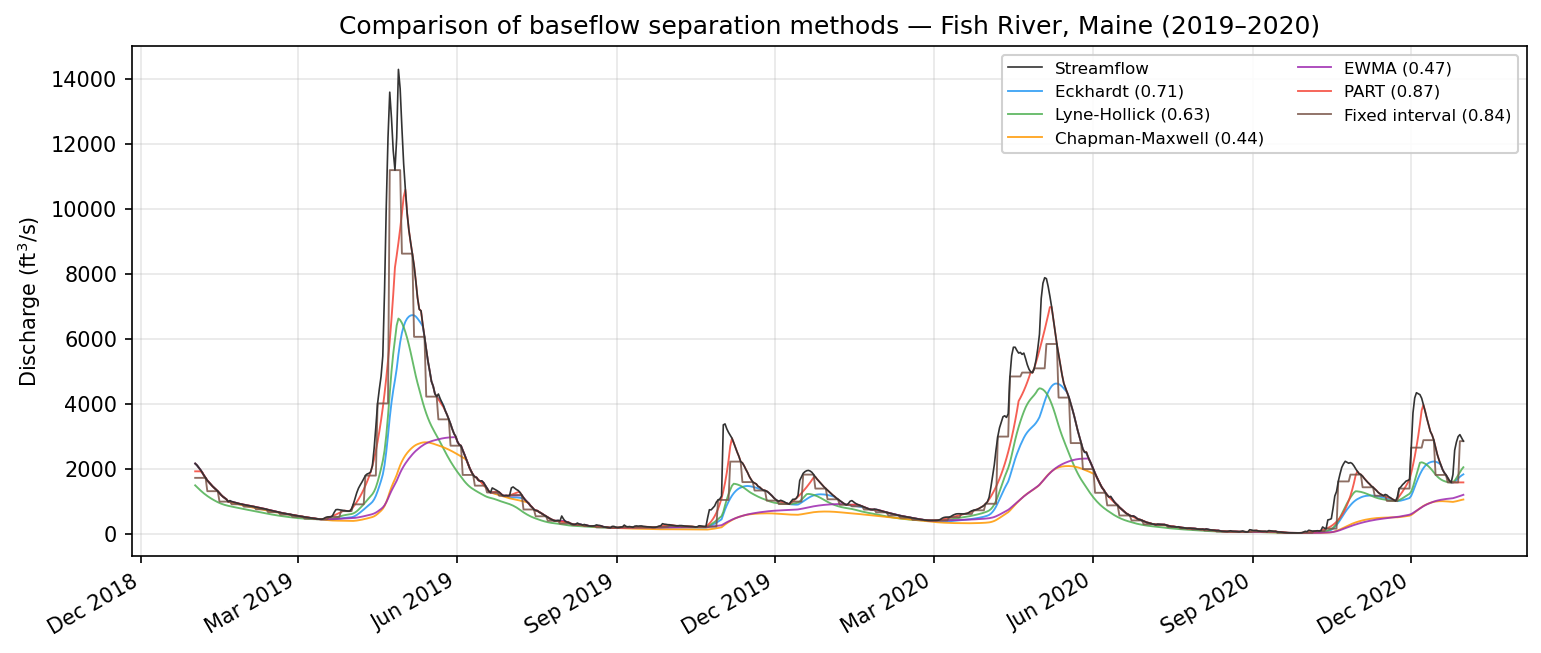
\includegraphics[width=\textwidth]{figures/overview_comparison.png}
\caption{Comparison of all 17 baseflow separation methods applied to Fish River (USGS 01013500), 2019--2020. Each panel shows the baseflow estimate with the corresponding BFI value.\label{fig:overview}}
\end{figure}

\subsection{Parameter Estimation}
\label{sec:param_estimation}

The recession coefficient $a$, required by most digital filter methods, can be estimated directly from the streamflow record:

\begin{lstlisting}[caption={Recession coefficient estimation.},label={lst:recession}]
from pybaseflow.estimate import recession_coefficient
a = recession_coefficient(Q, strict=True)
\end{lstlisting}

The function identifies strict baseflow periods (days on the recession limb where flow is declining monotonically) and computes the 5th percentile of the $-dQ/Q$ ratios to estimate the recession constant (Figure~\ref{fig:recession}).

For the Eckhardt filter, the $\mathrm{BFI_{max}}$ parameter can be set using the guidelines of Eckhardt~\cite{Eckhardt2005}: 0.80 for perennial streams with porous aquifers, 0.50 for ephemeral streams with porous aquifers, and 0.25 for perennial streams with hard-rock aquifers.

\begin{figure}[H]
\centering
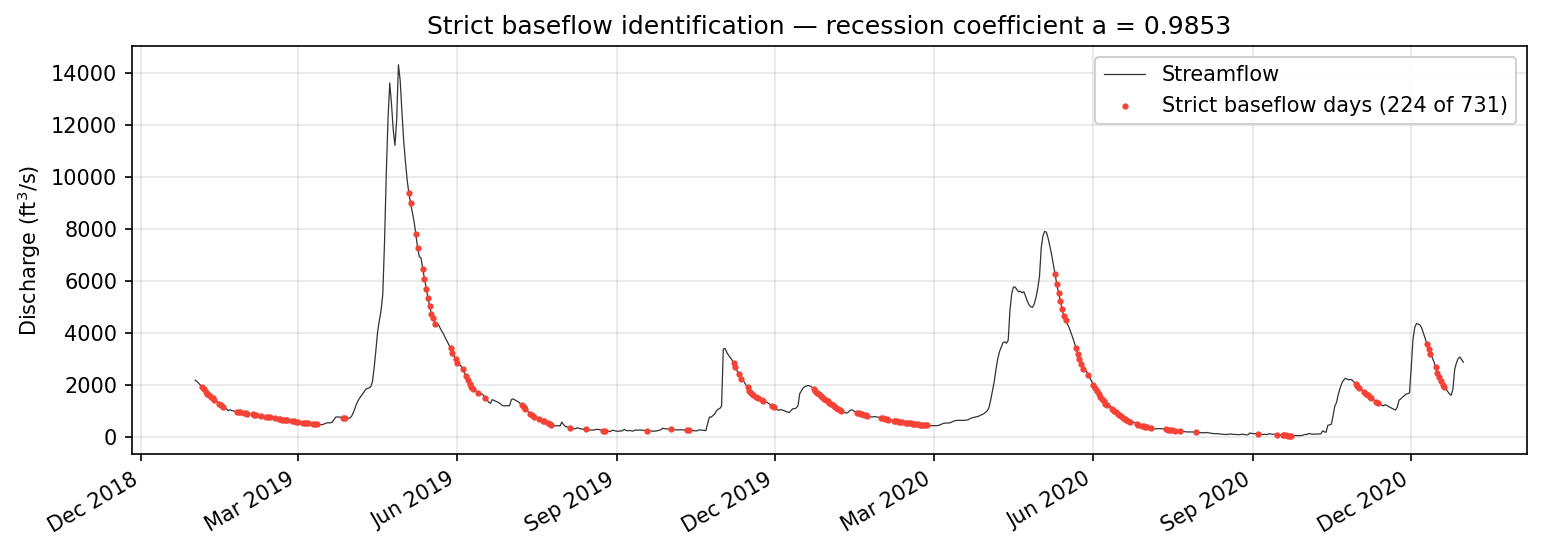
\includegraphics[width=0.85\textwidth]{figures/recession_coefficient.png}
\caption{Recession coefficient estimation showing identified strict baseflow periods (highlighted) and the fitted recession constant.\label{fig:recession}}
\end{figure}

\subsection{Tracer-Based Separation and Calibration}
\label{sec:cmb_example}

When specific conductance data are available, the CMB method provides a physically grounded separation:

\begin{lstlisting}[caption={CMB tracer-based separation and Eckhardt calibration.},label={lst:cmb}]
from pybaseflow.tracer import cmb, calibrate_eckhardt_from_cmb

# CMB separation
b_cmb = cmb(Q, SC, SC_BF=350, SC_RO=30)

# Use CMB result to calibrate Eckhardt's BFImax
BFImax_cal = calibrate_eckhardt_from_cmb(Q, b_cmb, a=a)
b_eck = pybaseflow.eckhardt(Q, a=a, BFImax=BFImax_cal)
\end{lstlisting}

Figure~\ref{fig:cmb} shows the CMB separation alongside the specific conductance time series and end-member reference lines.

\begin{figure}[H]
\centering
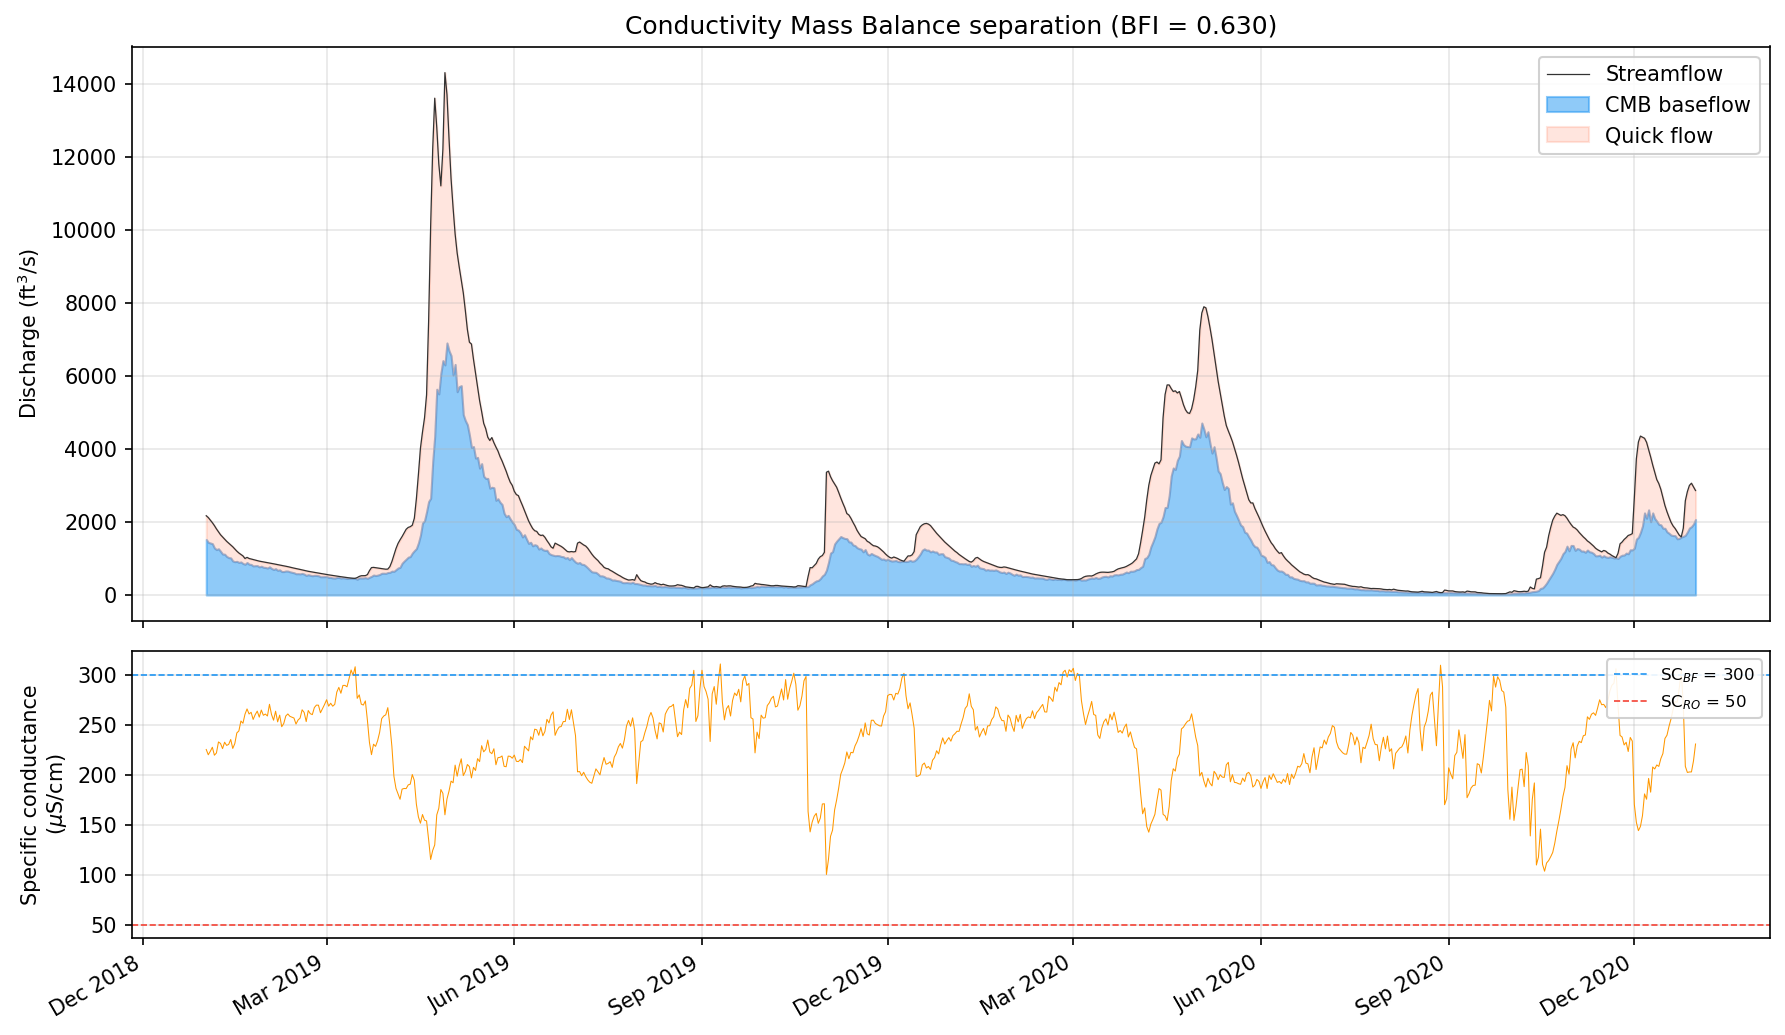
\includegraphics[width=0.85\textwidth]{figures/cmb.png}
\caption{Conductivity mass balance (CMB) baseflow separation. Top panel: streamflow with baseflow estimate. Bottom panel: specific conductance time series with $SC_{BF}$ and $SC_{RO}$ end-member lines.\label{fig:cmb}}
\end{figure}

%%%%%%%%%%%%%%%%%%%%%%%%%%%%%%%%%%%%%%%%%%
\section{Discussion}
\label{sec:discussion}

\subsection{Filter Family Taxonomy and Relationships}
\label{sec:taxonomy}

The generalized filter equation (Equation~\ref{eq:generalized}) provides a unifying lens through which to understand the relationships among recursive digital filters. Figure~\ref{fig:families} illustrates the structural difference between the two filter families during a peak flow event: the $\gamma = 0$ family (linear reservoir) responds only to the current streamflow, while the $\gamma = 1$ family (signal processing) incorporates a moving average of streamflow, producing different recession characteristics.

\begin{figure}[H]
\centering
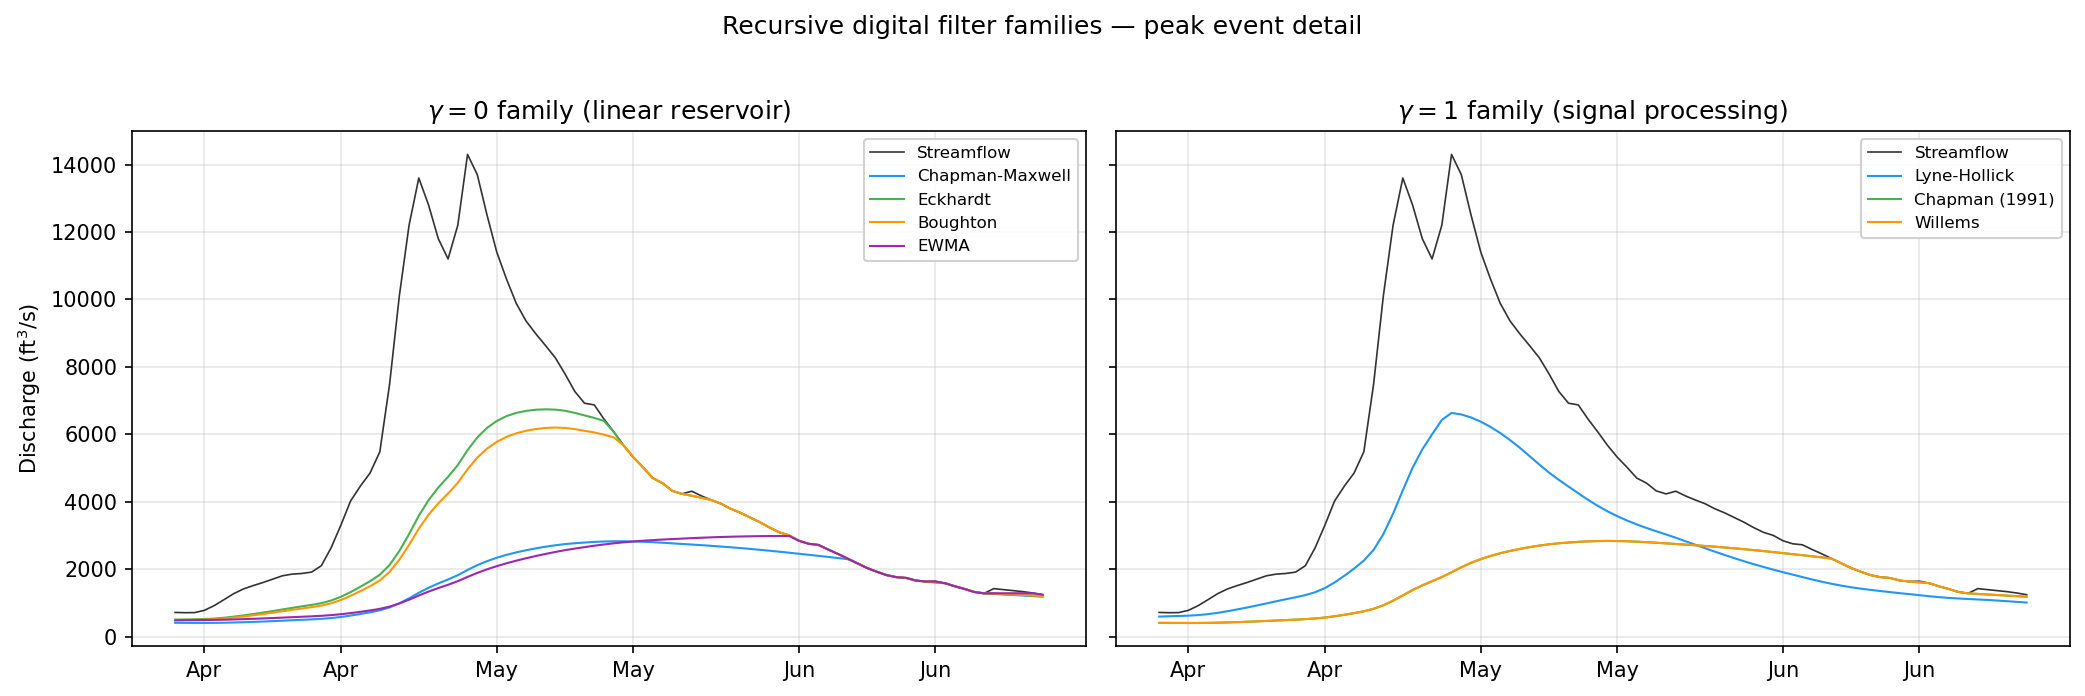
\includegraphics[width=0.85\textwidth]{figures/filter_families.png}
\caption{Comparison of $\gamma = 0$ (linear reservoir) and $\gamma = 1$ (signal processing) filter families applied to a peak flow event, illustrating the structural difference in how each family partitions the hydrograph.\label{fig:families}}
\end{figure}

The IHACRES filter~\cite{Jakeman1993} occupies a unique position as a bridge between the two families. Its $\gamma = \alpha_s$ parameter allows continuous interpolation between the Boughton filter ($\alpha_s = 0$, pure $\gamma = 0$ behavior) and the signal-processing family ($\alpha_s \to -1$). Figure~\ref{fig:ihacres_sensitivity} demonstrates this transition, showing how the baseflow estimate varies as $\alpha_s$ changes from 0 to $-0.9$.

\begin{figure}[H]
\centering
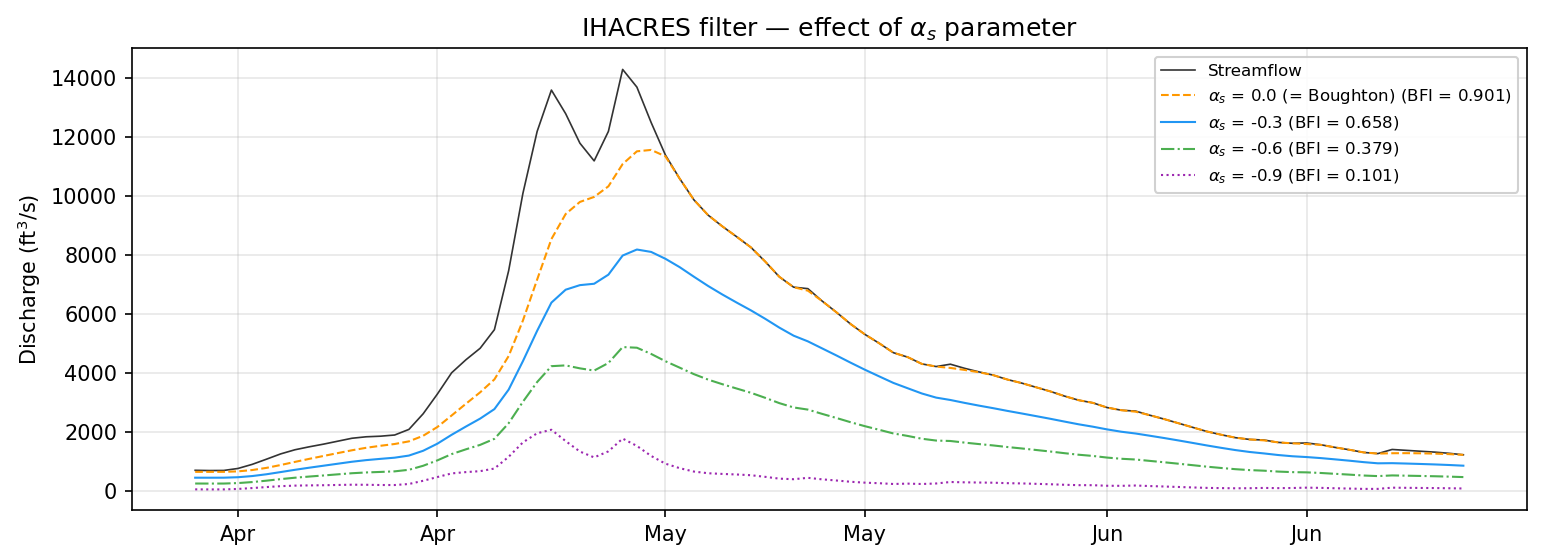
\includegraphics[width=0.85\textwidth]{figures/ihacres_sensitivity.png}
\caption{Sensitivity of the IHACRES filter to the $\alpha_s$ parameter, showing the transition from $\gamma = 0$ family behavior ($\alpha_s = 0$, equivalent to Boughton) toward $\gamma = 1$ family behavior ($\alpha_s \to -1$).\label{fig:ihacres_sensitivity}}
\end{figure}

The algebraic equivalence between the Boughton and Eckhardt filters---related by $C = (1-a)\cdot\mathrm{BFI_{max}}/(1-\mathrm{BFI_{max}})$---means that the Eckhardt filter, which is parameterized in terms of the physically interpretable $\mathrm{BFI_{max}}$, subsumes both the Boughton and Chapman--Maxwell filters (the latter being the special case $\mathrm{BFI_{max}} = 0.5$).

\subsection{Comparison with Existing Tools}
\label{sec:comparison_tools}

Table~\ref{tab:comparison} compares \texttt{pybaseflow} with existing baseflow separation tools.

\begin{table}[H]
\caption{Comparison of \texttt{pybaseflow} with existing baseflow separation tools.\label{tab:comparison}}
\small
\begin{tabularx}{\textwidth}{lcccc}
\toprule
\textbf{Feature} & \textbf{pybaseflow} & \textbf{HYSEP/PART} & \textbf{WHAT} & \textbf{baseflow}~\cite{Xie2020} \\
\midrule
Language & Python & Fortran & Web & Python \\
Methods & 17 & 4 & 3 & 11 \\
Scriptable/automatable & Yes & Limited & No & Yes \\
Tracer-based methods & Yes & No & No & No \\
USGS data retrieval & Yes & No & Yes & No \\
pip-installable & Yes & No & No & Yes \\
Active documentation & Yes & No & Yes & No \\
Unified filter framework & Yes & N/A & No & No \\
\bottomrule
\end{tabularx}
\end{table}

\subsection{Limitations}
\label{sec:limitations}

Several limitations should be noted. The package currently operates on daily time-step data only; sub-daily or monthly applications would require adaptation. All methods operate on single-station time series; spatial interpolation of baseflow across a watershed is not supported. The recursive digital filters are deterministic and do not provide uncertainty estimates. For the CMB method, the assumption of two end-members and conservative mixing may not hold in all hydrogeological settings. Furthermore, as Zhang et al.~\cite{Zhang2021} demonstrated, calibrating Eckhardt filter parameters from CMB-derived baseflow works well at annual scales but can perform poorly at daily scales, and users should be aware of this limitation.

\subsection{Future Development}
\label{sec:future}

Planned future development includes support for sub-daily time steps, automated method selection algorithms, uncertainty quantification for filter-based methods, integration of additional tracer types (e.g., stable isotopes), and spatial baseflow mapping using gridded data.

%%%%%%%%%%%%%%%%%%%%%%%%%%%%%%%%%%%%%%%%%%
\section{Conclusions}
\label{sec:conclusions}

We have presented \texttt{pybaseflow}, an open-source Python package that unifies 17 baseflow separation methods under a consistent API. The package spans four methodological paradigms---recursive digital filters, graphical methods, recession analysis, and tracer-based approaches---making it the most comprehensive Python tool available for baseflow separation.

A key theoretical contribution is the identification of a generalized three-parameter recursive digital filter equation (Equation~\ref{eq:generalized}) that reveals the algebraic relationships among 11 popular methods, including the equivalence of the Boughton and Eckhardt filters and the bridging role of IHACRES between the two filter families. The package also provides the first Python implementation of the USGS PART method and a novel CMB-to-Eckhardt calibration bridge linking tracer measurements to digital filter parameters.

The package is designed for ease of use: it is pip-installable, provides built-in USGS data retrieval, includes bundled sample data, and is accompanied by comprehensive documentation with method guides and worked examples. We hope that \texttt{pybaseflow} will serve as a practical tool for hydrologists, water resource engineers, and researchers, and that its open-source nature will foster community contributions and continued development.

%%%%%%%%%%%%%%%%%%%%%%%%%%%%%%%%%%%%%%%%%%
\vspace{6pt}

%%%%%%%%%%%%%%%%%%%%%%%%%%%%%%%%%%%%%%%%%%
%% optional
%\supplementary{The following supporting information can be downloaded at: \linksupplementary{s1}}

%%%%%%%%%%%%%%%%%%%%%%%%%%%%%%%%%%%%%%%%%%
\authorcontributions{Conceptualization, N.J. and T.P.C.; methodology, X.L. and A.A.; software, X.L., A.A., J.H., A.K. and B.B.; validation, X.L. and A.A.; writing---original draft preparation, X.L.; writing---review and editing, N.J., G.W., D.R. and T.P.C.; supervision, N.J. and T.P.C. All authors have read and agreed to the published version of the manuscript.}

\funding{This research received no external funding.}

%\informedconsent{}

\dataavailability{The \texttt{pybaseflow} Python package is publicly available at \url{https://github.com/BYU-Hydroinformatics/pybaseflow}. Documentation is available at \url{https://pybaseflow.readthedocs.io/en/latest/}. The bundled sample dataset originates from USGS station 01013500 (Fish River near Fort Kent, Maine).}

\conflictsofinterest{The authors declare no conflicts of interest.}

%%%%%%%%%%%%%%%%%%%%%%%%%%%%%%%%%%%%%%%%%%
\begin{adjustwidth}{-\extralength}{0cm}

\reftitle{References}

\begin{thebibliography}{99}

\bibitem{Arnold1999}
Arnold, J.G.; Allen, P.M. Automated Methods for Estimating Baseflow and Ground Water Recharge from Streamflow Records. \textit{J. Am. Water Resour. Assoc.} \textbf{1999}, \textit{35}, 411--424. \url{https://doi.org/10.1111/j.1752-1688.1999.tb03599.x}

\bibitem{Barnes1939}
Barnes, B.S. The Structure of Discharge-Recession Curves. \textit{Trans. Am. Geophys. Union} \textbf{1939}, \textit{20}, 721--725.

\bibitem{Boughton1993}
Boughton, W.C. A Hydrograph-Based Model for Estimating the Water Yield of Ungauged Catchments. In Proceedings of the Hydrology and Water Resources Symposium; Institution of Engineers Australia: Newcastle, Australia, 1993; pp.~317--324.

\bibitem{Chapman1991}
Chapman, T.G. Comment on ``Evaluation of Automated Techniques for Base Flow and Recession Analyses'' by R.~J.~Nathan and T.~A.~McMahon. \textit{Water Resour. Res.} \textbf{1991}, \textit{27}, 1783--1784. \url{https://doi.org/10.1029/91WR01007}

\bibitem{ChapmanMaxwell1996}
Chapman, T.G.; Maxwell, A.I. Baseflow Separation---Comparison of Numerical Methods with Tracer Experiments. In Proceedings of the Hydrology and Water Resources Symposium; Institution of Engineers Australia: Hobart, Australia, 1996; pp.~539--545.

\bibitem{Cheng2016}
Cheng, L.; Zhang, L.; Brutsaert, W. Automated Selection of Pure Base Flows from Regular Daily Streamflow Data: Objective Algorithm. \textit{J. Hydrol. Eng.} \textbf{2016}, \textit{21}, 06016008. \url{https://doi.org/10.1061/(ASCE)HE.1943-5584.0001427}

\bibitem{Eckhardt2005}
Eckhardt, K. How to Construct Recursive Digital Filters for Baseflow Separation. \textit{Hydrol. Process.} \textbf{2005}, \textit{19}, 507--515. \url{https://doi.org/10.1002/hyp.5675}

\bibitem{Furey2001}
Furey, P.R.; Gupta, V.K. A Physically Based Filter for Separating Base Flow from Streamflow Time Series. \textit{Water Resour. Res.} \textbf{2001}, \textit{37}, 2709--2722. \url{https://doi.org/10.1029/2001WR000243}

\bibitem{Jakeman1993}
Jakeman, A.J.; Hornberger, G.M. How Much Complexity Is Warranted in a Rainfall-Runoff Model? \textit{Water Resour. Res.} \textbf{1993}, \textit{29}, 2637--2649. \url{https://doi.org/10.1029/93WR00877}

\bibitem{Lim2005}
Lim, K.J.; Engel, B.A.; Tang, Z.; Choi, J.; Kim, K.; Muthukrishnan, S.; Tripathy, D. Automated Web GIS Based Hydrograph Analysis Tool, WHAT. \textit{J. Am. Water Resour. Assoc.} \textbf{2005}, \textit{41}, 1407--1416. \url{https://doi.org/10.1111/j.1752-1688.2005.tb03808.x}

\bibitem{Lyne1979}
Lyne, V.; Hollick, M. Stochastic Time-Variable Rainfall-Runoff Modelling. In Proceedings of the Hydrology and Water Resources Symposium; Institution of Engineers Australia: Perth, Australia, 1979; pp.~89--93.

\bibitem{Nathan1990}
Nathan, R.J.; McMahon, T.A. Evaluation of Automated Techniques for Base Flow and Recession Analyses. \textit{Water Resour. Res.} \textbf{1990}, \textit{26}, 1465--1473. \url{https://doi.org/10.1029/WR026i007p01465}

\bibitem{Rutledge1998}
Rutledge, A.T. Computer Programs for Describing the Recession of Ground-Water Discharge and for Estimating Mean Ground-Water Recharge and Discharge from Streamflow Records---Update; \textit{U.S. Geological Survey Water-Resources Investigations Report 98-4148}; USGS: Reston, VA, USA, 1998.

\bibitem{Sloto1996}
Sloto, R.A.; Crouse, M.Y. HYSEP---A Computer Program for Streamflow Hydrograph Separation and Analysis; \textit{U.S. Geological Survey Water-Resources Investigations Report 96-4040}; USGS: Lemoyne, PA, USA, 1996.

\bibitem{Spongberg2000}
Spongberg, M.E. Spectral Analysis of Base Flow Separation with Digital Filters. \textit{Water Resour. Res.} \textbf{2000}, \textit{36}, 745--752. \url{https://doi.org/10.1029/1999WR900303}

\bibitem{Stewart2007}
Stewart, M.T.; Cimino, J.; Ross, M. Calibration of Base Flow Separation Methods with Streamflow Conductivity. \textit{Groundwater} \textbf{2007}, \textit{45}, 17--27. \url{https://doi.org/10.1111/j.1745-6584.2006.00263.x}

\bibitem{Tularam2008}
Tularam, G.A.; Ilahee, M. Exponential Smoothing Method of Base Flow Separation and Its Impact on Continuous Loss Estimates. \textit{Am. J. Environ. Sci.} \textbf{2008}, \textit{4}, 136--144. \url{https://doi.org/10.3844/ajessp.2008.136.144}

\bibitem{UKIH1980}
Institute of Hydrology. \textit{Low Flow Studies}; Institute of Hydrology: Wallingford, UK, 1980.

\bibitem{Willems2009}
Willems, P. A Time Series Tool to Support the Multi-Criteria Performance Evaluation of Rainfall-Runoff Models. \textit{Environ. Model. Softw.} \textbf{2009}, \textit{24}, 311--321. \url{https://doi.org/10.1016/j.envsoft.2008.09.005}

\bibitem{Xie2020}
Xie, J.; Liu, X.; Wang, K.; Yang, T.; Liang, K.; Liu, C. Evaluation of Typical Methods for Baseflow Separation in the Contiguous United States. \textit{J. Hydrol.} \textbf{2020}, \textit{583}, 124628. \url{https://doi.org/10.1016/j.jhydrol.2020.124628}

\bibitem{Zhang2021}
Zhang, J.; Song, J.; Cheng, L.; Zheng, H.; Wang, Y.; Huai, B.; Sun, W.; Qi, S.; Zhao, P.; Wang, Y.; Li, Q. Can the Two-Parameter Recursive Digital Filter Really Be Calibrated by the Conductivity Mass Balance Method? \textit{Hydrol. Earth Syst. Sci.} \textbf{2021}, \textit{25}, 1747--1760. \url{https://doi.org/10.5194/hess-25-1747-2021}

\end{thebibliography}

\end{adjustwidth}

\end{document}
